\vspace{-0.3cm}
\subsection*{Tables and Keys}
\vspace{-0.1cm}

\begin{center}
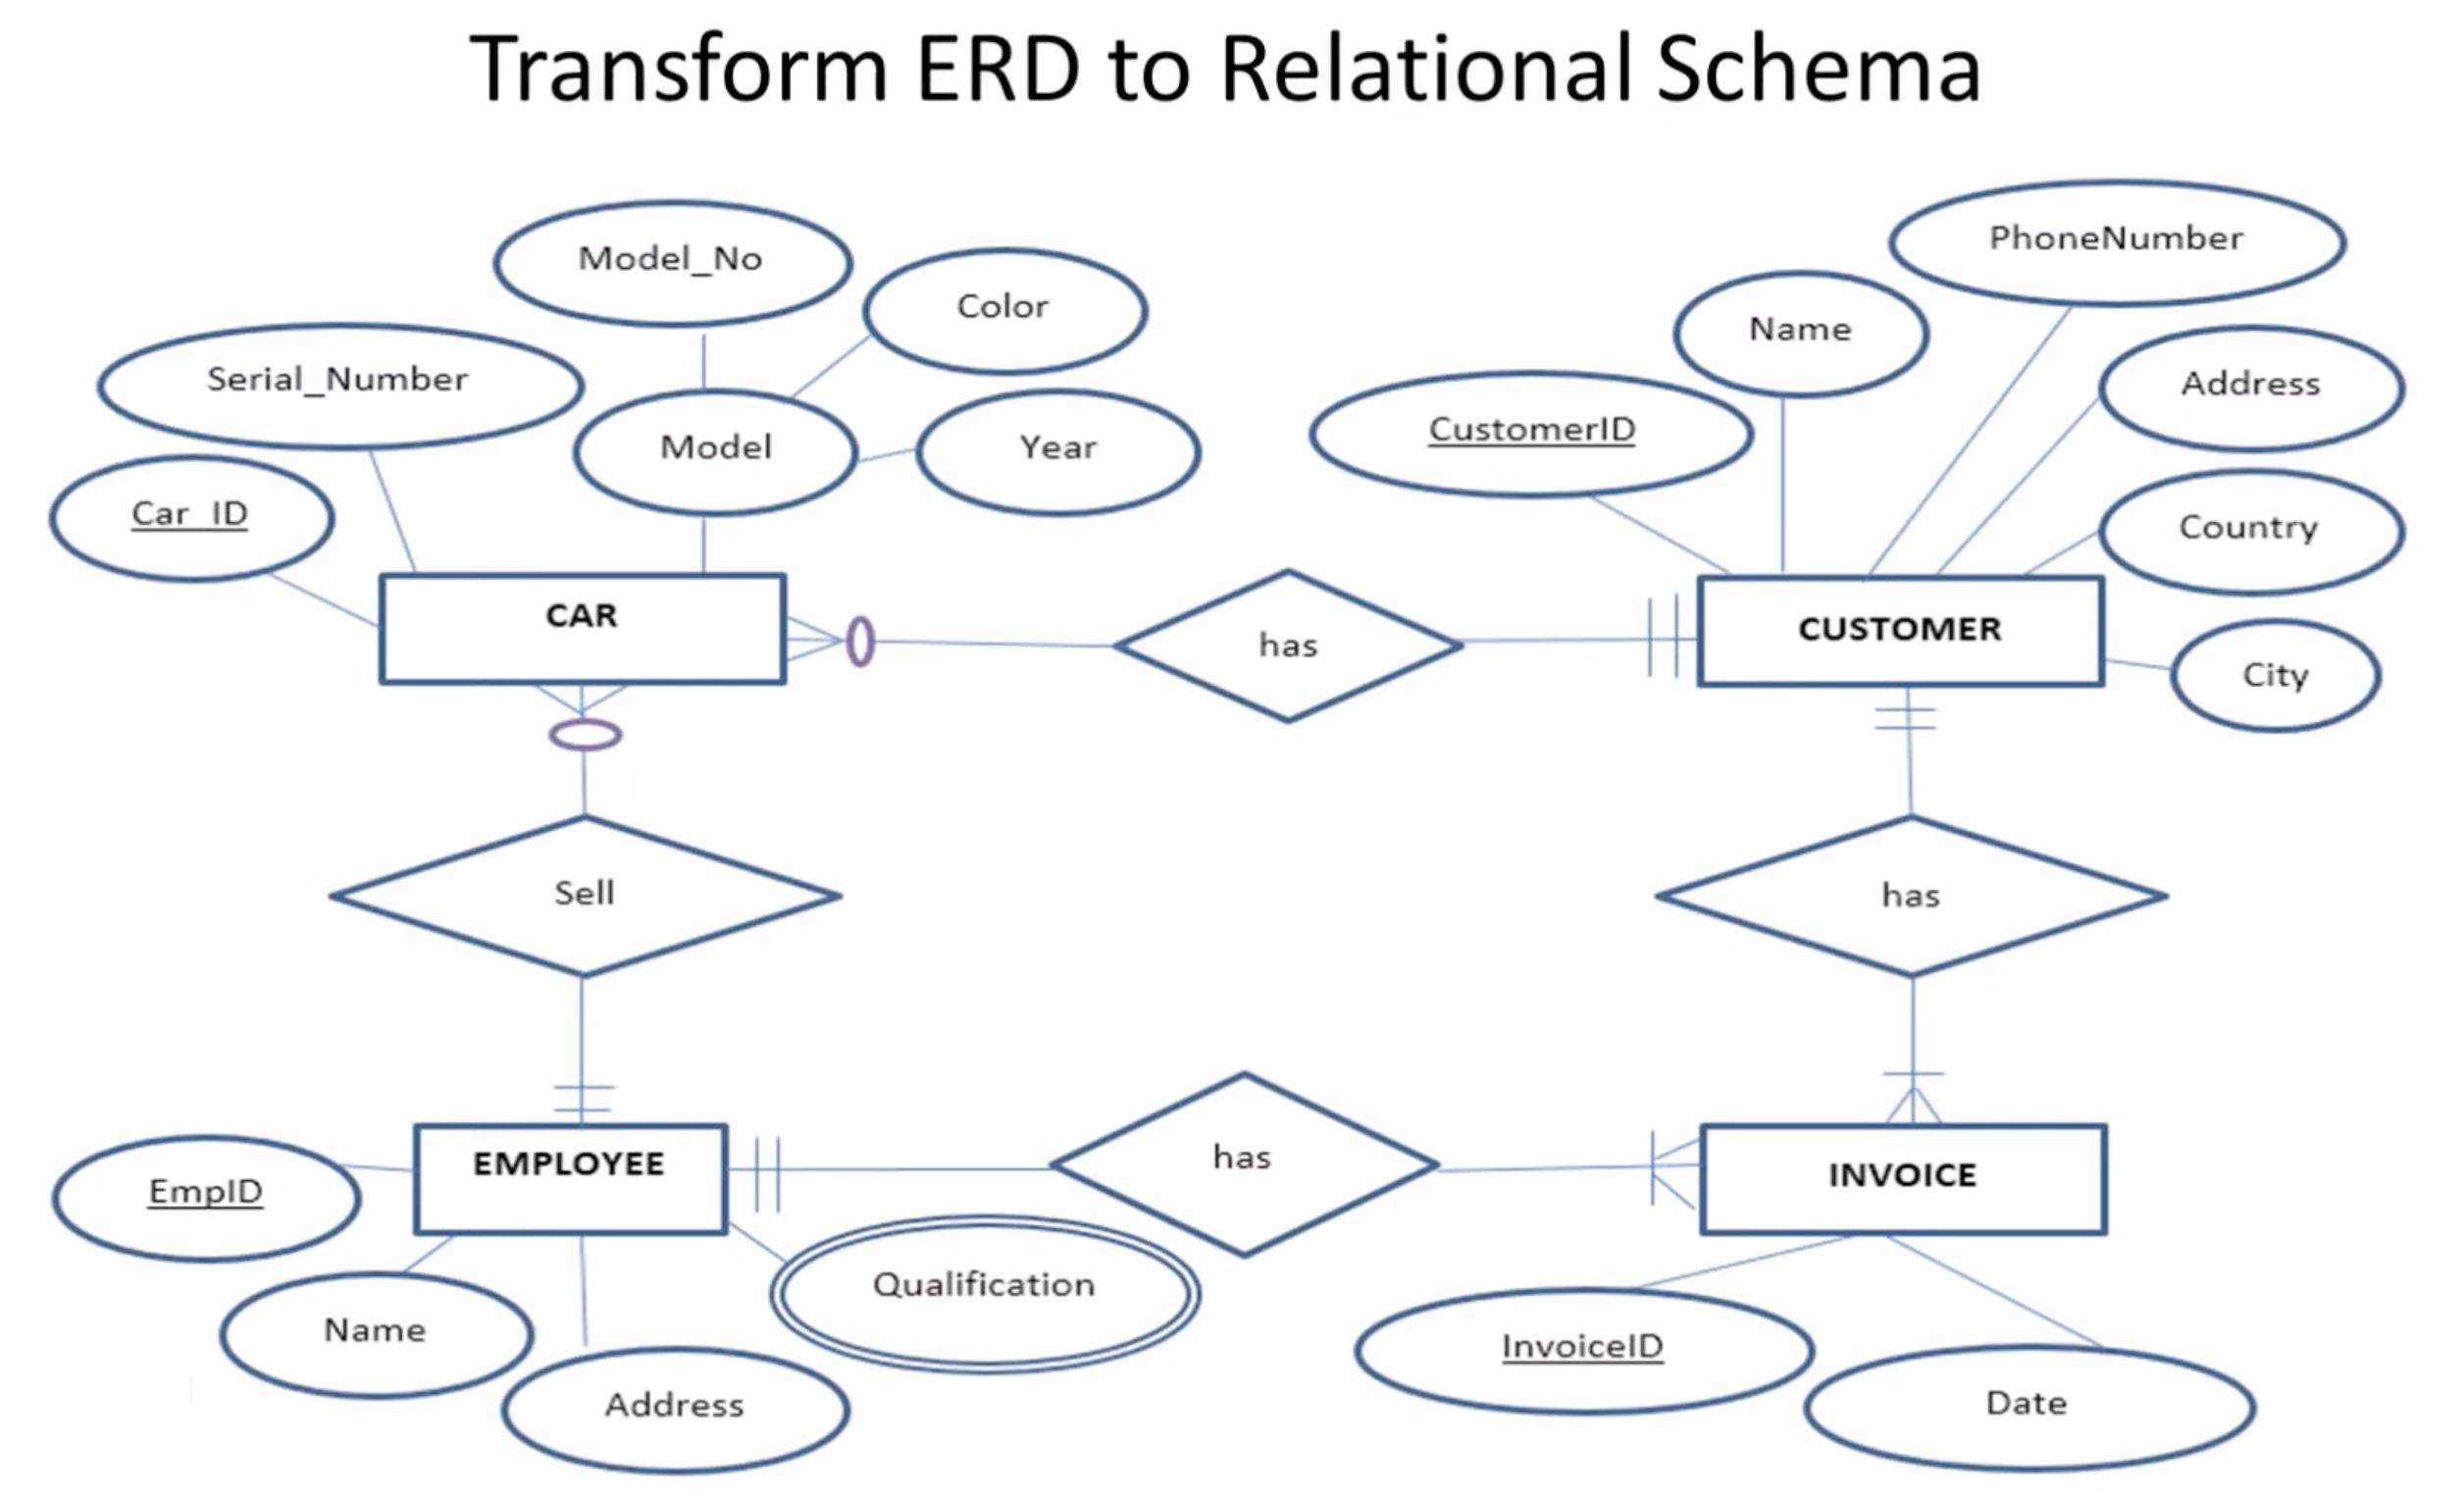
\includegraphics[width=8cm,height=4cm]{logical_model/entity_relation_img}
\end{center}

\vspace{-0.1cm}

\begin{itemize}[noitemsep,leftmargin=*]
\leftskip-\dimexpr\leftmargin %%%
    \item[] \textbf{CAR} table with primary key \textit{Car\_ID}.
    \item[] \textbf{CUSTOMER} table with primary key \textit{CustomerID}.
    \item[] \textbf{EMPLOYEE} table with primary key \textit{EmpID}.
    \item[] \textbf{INVOICE} table with primary key \textit{InvoiceID}, including foreign key \textit{CustomerID}.
    \item[] \textbf{SELL} join table to represent the many-to-many relationship between \textbf{CAR} and \textbf{EMPLOYEE}.
\end{itemize}

\noindent
\begin{minipage}[t]{.5\linewidth}
    \centering
    \begin{tabular}{ll}
        \toprule
        \textbf{CAR} & \\
        \midrule
        Car\_ID & Primary Key \\
        Serial\_Number & \\
        Model & \\
        Model\_No & \\
        Color & \\
        Year & \\
        \bottomrule
    \end{tabular}
\end{minipage}%
\begin{minipage}[t]{.5\linewidth}
    \centering
    \begin{tabular}{ll}
        \toprule
        \textbf{CUSTOMER} & \\
        \midrule
        CustomerID & Primary Key \\
        Name & \\
        PhoneNumber & \\
        Address & \\
        Country & \\
        City & \\
        \bottomrule
    \end{tabular}
\end{minipage}


\noindent
\begin{minipage}[t]{.5\linewidth}
    \centering
    \begin{tabular}{ll}
        \toprule
        \textbf{EMPLOYEE} & \\
        \midrule
        EmpID & Primary Key \\
        Name & \\
        Address & \\
        Qualification & \\
        \bottomrule
    \end{tabular}
\end{minipage}%
\begin{minipage}[t]{.5\linewidth}
    \centering
    \begin{tabular}{ll}
        \toprule
        \textbf{INVOICE} & \\
        \midrule
        InvoiceID & Primary Key \\
        Date & \\
        CustomerID & Foreign Key \\
        \bottomrule
    \end{tabular}
\end{minipage}%

% SELL Join Table
\begin{table}[h!]
    \centering
    \begin{tabular}{ll}
        \toprule
        \textbf{SELL} & \\
        \midrule
        Car\_ID & Foreign Key (References CAR) \\
        EmpID & Foreign Key (References EMPLOYEE) \\
        Sell\_Details & Additional information about the sale \\
        \bottomrule
    \end{tabular}
\end{table}